\chapter{Safety}
\begin{figure}[h]
\centering
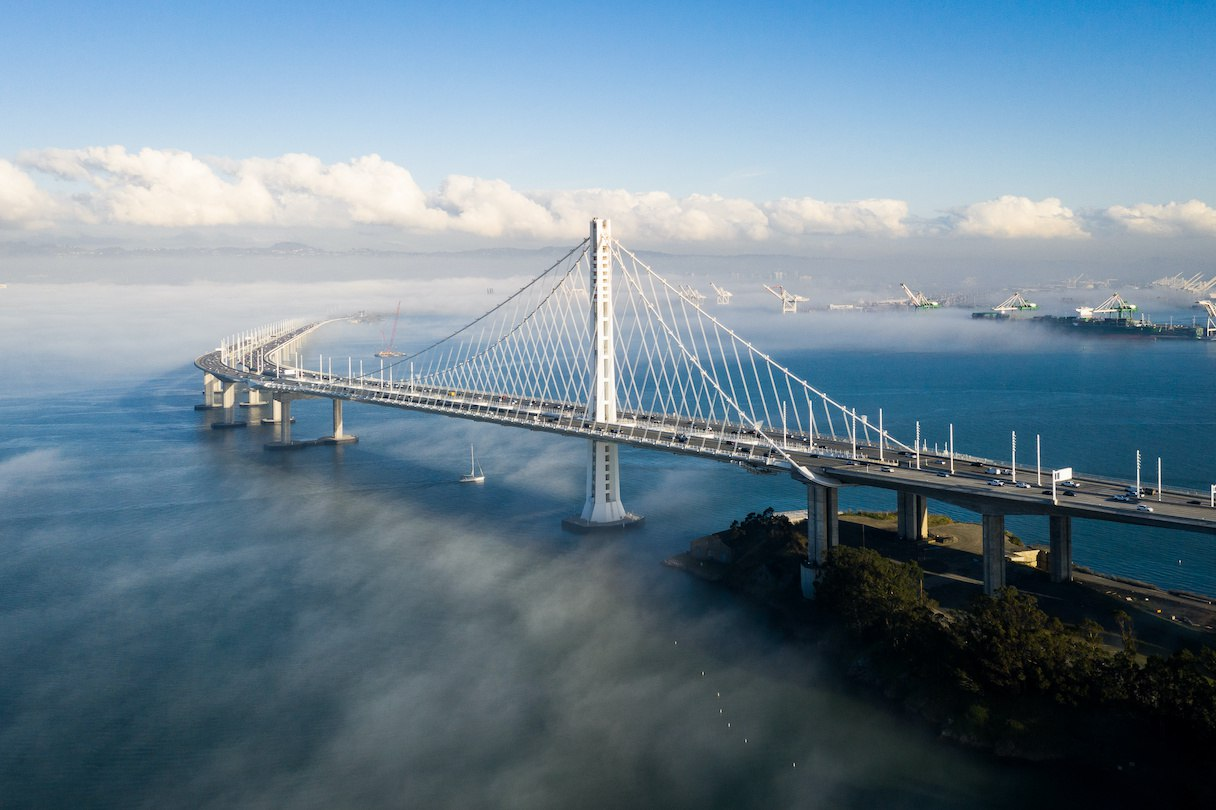
\includegraphics[width=0.8\textwidth]{Capitoli_Report/4.1_Safety.png}
\caption{\cite{picsafety}}
\label{fig:safety}
\end{figure}
\newpage
\section{Introduction}
The case study regards the discussion of a \textit{fictional case of liberty limitation techno-regulation} in transportation, which is the implementation of the \textbf{Intelligent Decibel Lowering Engine Restrainer} (IDLER) on all new motorcycles. This is a device that allows to automatically limit the engine's maximum RPM, in order to reduce the (excessive) emitted noise in certain locations, thanks to a GPS installed on board.

\emph{(65 words)}

\section{What are the two most convincing arguments \textit{in favor of obligating} the implementation of IDLER, in your opinion?}
\subsection{Public nuisance}
On certain roads or in urban centers there can be a very intense traffic of motorcycles, since they could be near places that are very attractive for motorcyclists: roads bordering a lake or mountain passes are all places where it can be very pleasant to ride, as they are very engaging from the driver's point of view. For this reason, the constant passage of motorcycles could become very annoying for the inhabitants of those places and disturb their quietness, especially during the weekends. Therefore, as there are already regulations that prohibit to honk in the cities or to make noises late at night, the introduction of a device such as IDLER could be considered to better preserve and guarantee public peace. In addition, WHO classifies as "harmful" every sound above 75 dB, and almost all bikes can go beyond this limit.

\subsection{Pollutant emissions}
When going at high speed and high RPM, the engine produces lots of pollutant emissions, so its introduction could also help from the point of view of reducing them, especially in the city center, where this problem is more present than other places.

\emph{(198 words)}

\section{What are the two most convincing arguments \textit{against obligating} the implementation of IDLER, in your opinion?}
\subsection{Limited driving experience}
Usually, high-performance and sport motorcycles, with a particularly loud exhaust sound, are mainly purchased by enthusiasts to use them specifically on the roads mentioned above: in these cases, sound plays an active role in driving involvement, so its attenuation or elimination could be seen as a limitation to one's passion and, consequently, to one's freedom.

\subsection{Low flexibility in case of emergency}
Other problems may arise if the driver needs to move faster than the IDLER allows, due to a sudden need or emergency. As an extreme consequence, this could also lead to people not buying these type of vehicles, decreasing the  motorcycles' selling. Another aspect to be considered is the nature of the motorcycle itself. To negotiate a curve, a motorbike of any sort needs a given speed to generate the forces that make the leaning equilibrium possible. If, for any reason (GPS malfunctioning, bad tuning of the interested zones, IDLER malfunctioning and similar), the IDLER would cut power while curving, this can lead to a loss of control and eventually even to a crash.

\emph{(172 words)}

\section{Considering the previous arguments, are you in favor or against the obligatory implementation of IDLER? And \textit{why}?}
The implementation of some device to reduce acoustic pollution is something that any motorcyclist would approve, if he/she was the one suffering the discomfort. What makes IDLER not the best solution, however, is the lack of controllability; GPS is not an accurate system, so errors in the position estimation can lead to dangerous situations.

A solution that can make the IDLER's philosophy applicable is to couple it with some ad hoc legislation and infrastructure.
One example can be the implementation of an IDLER that switches on based on signals coming from sensorized roads only in proximity of points of interest (like hospitals and schools). These conditions must be adequately marked by signage, so that the rider is prepared for the fact that the bike will suddenly lose power. Another aspect to consider is personal responsibility. Motorcycles tend to produce the most noise when the engine RPMs are high and that, in most of real-life scenarios, corresponds to the bike going fast. By introducing speed limits, combined with some effective speed radars targeted to specific zones like the aforementioned, IDLER will maybe not even be necessary.

In conclusion, IDLER is an interesting solution; it makes riders renounce to a trivial pleasure like the sound of a high revving bike for a great public good. However, how to apply this concept is something that needs some further analysis to give the best solution.

\emph{(213 words)}

\emph{(549 total words)}

\begin{comment}
\begin{thebibliography}{99}

\bibitem[Fahlquist, 2009]{p1}
Fahlquist, J. N. (2009)

\textit{Saving lives in road traffic-ethical aspects.}

\textbf{Journal of Public Health, 17(6)}

\bibitem[Smids, 2018]{p2}
Smids, J. (2018)

\textit{The moral case for intelligent speed adaptation.}

\textbf{Journal of Applied Philosophy, 35(2)}

\end{thebibliography}

\textit{Document write with \LaTeX. Template founded on Overleaf} (\textbf{Copyright (c) 2020 George Kour}).
\end{comment}